Now we discuss in details our semantic interpretation of the AGREE contracts with scheduled components.
\begin{figure}[ht!]
\centering
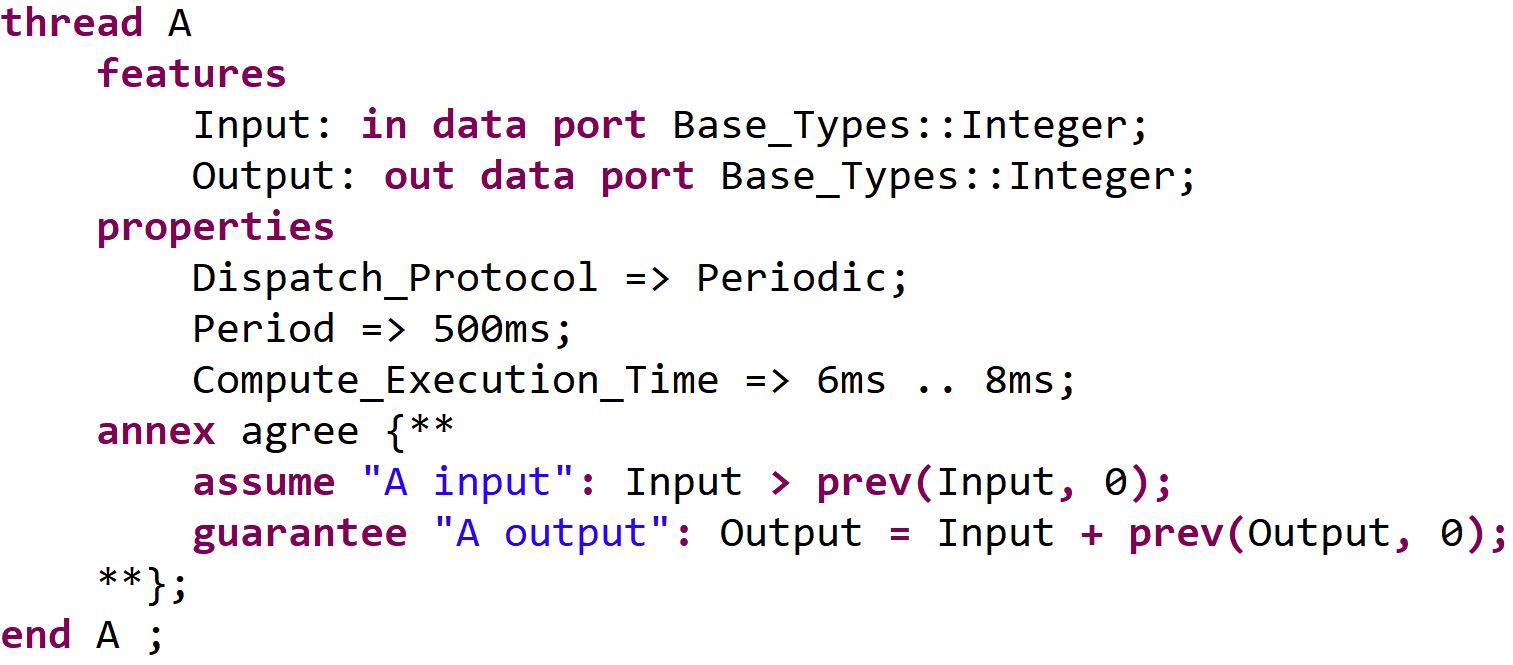
\includegraphics[width=80mm]{pre.jpg}
\caption{A Simple Integrator AADL Model in AGREE\label{integratorFig}}
\end{figure}

Consider the AADL model of an integrator, shown in Figure \ref{integratorFig}. We assume an execution time slot is assigned to the thread.  
The first question we face is when the contracts shall hold. In a synchronous model, contracts hold at every instant. However, with scheduled execution, it is reasonable to assume the contract may not hold when the component is not activated. But once it is activated, shall they hold throughout the whole execution or just at certain instants? Second, how shall $Input$ referred in the contract be interpreted? One interpretation is that it refers to the input value at the time when the contract is evaluated, which may vary during the execution. Another interpretation is that it refers to the input value when the component starts its execution. In other words, there is a notion of \emph{sample and hold}. This interpretation is consistent with the \emph{frozen} inputs described in the AADL V2 standard. Third, how the \emph{prev} operator shall be interpreted? In a synchronous model, it refers to the previous instant. However, with scheduled execution, it seems reasonable to interpret \emph{prev} as previous activation (i.e. the last value when the component was activated). If the contracts hold throughout the activation, a more sensible interpretation is that at the first instant during activation, it refers to the previous activation. Then at each following instant, it refers to the last updated value in the current activation. This interpretation is adopted in the \emph{activation condition} in SCADE \cite{scade} or the \emph{clock} mechanism in SIGNAL \cite{signal}.

AGREE contracts are intended to descirbe system or component requirements \cite{AGREE2}, and therefore provide abstractions of the implementations. Guarantees usually model the component requirements and assumptions model the environmental constraints for the component. Following the AADL \emph{input-compute-output} model, we interpret that the assumptions shall hold at the start of the execution (i.e. \emph{dispatch}) when the inputs are read in. The guarantees shall be satisfied at the end of the execution (i.e. \emph{complete}) when the outputs are written. This interpretation has a few implications. 
First, since we adopt the AADL frozen inputs concept, any reference to $Input$ refers to the input value that was read in at dispatch.
Second, a component's assigned time slot does not necessarily match exactly its execution time window. If the time slot is greater than its execution time, we interpret the start and end of the time slot as dispatch and complete, respectively. Otherwise, we interpret a preemption has occurred.
Third, each contract is examined exactly once in each activation. Thus, we interpret the $prev$ operator as the previous activation. 
Fourth, the guarantees are not models of the \emph{transient} behavior during an execution. Instead, we interpret them as constraints on the \emph{steady-state} outputs at the end of activation.

%This is different from the real-time behavior models used to formalize AADL semantics, like real-time Maude \cite{maude}, timed automata \cite{behaviorannex}, and timed Petri net \cite{tpn}. They model the component timing behavior throughout the whole execution. 
%We assume the requirements do not contain real-time constraints. Modeling such constraints in AGREE is discussed in \cite{rtAGREE}.
AGREE contracts may include discrete time-based requirements. In practice, a timer is usually implemented as a counter whose limit (constant) can be calculated based on the frequency of component execution. The counter is activated periodically and increments during each activation independent of the execution time. 
Modeling continuous-valued real-time constraints in AGREE is discussed in \cite{rtAGREE}.
%This is consistent with our interpretation.

We introduce two new events \emph{dispatch} and \emph{complete} for each component to model the start and end of its activation, respectively. 
Similarly, for a system (consists of components), the two events model the start and end of a scheduling cycle. 
The two events shall appear in pairs and alternately. \emph{dispatch} shall appear before \emph{complete}. We will introduce the notion of \emph{well-ordered} to capture the pattern.

In SCADE and SIGNAL, when a component is not activated, its outputs keep their previous values. We extend the output freeze time window to between \emph{complete} events, including activation. We understand in practice, the actual output values may change during activation. We choose this because we interpret the \emph{guarantees} as steady-state requirements of outputs at \emph{complete}. The outputs values between dispatch and complete is undefined. Thus, we model them with the last outputs values, so that the outputs have well-defined behavior at every instant.

We inherit the same notion of composition used in the current AGREE framework. A connection between two components means their contracts refer to the same variable. 
This, combined with a schedule, essentially simulates asynchronous communication between components through a \emph{shared variable}. 
%This is consistent with the AADL data port sampling semantics. 
We consider single-machine schedules. The scheduler ensures at most one component is activated at a time. For a preemptive schedule, we require a component can only be preempted by another component if they do not have connections. Thus, there is no ambiguity on the order of read and write or the variable value referenced in the contracts.
The communication channel may also be viewed as a buffer or queue of size one. %The writer overwrites when overflow occurs. The reader reads the last value if the buffer is empty. 
This means the proposed model only supports limited AADL event data port communication.
 
We assume the system-level inputs do not change values when the ultimate destination component is activated. In practice, this means there may exist a queue that stores the system-level input messages, which are periodically sampled by the components. Or the inputs may come from another system, which is inactive while the system is active.

The inputs freeze rule may imply the assumptions could be examined at \emph{complete}, instead of \emph{dispatch}. Thus, we may not need the \emph{dispatch} event. We keep it mainly due to two considerations. First, the assumptions in general could depend on the past outputs. And the outputs are updated at \emph{complete}. So the outputs values at \emph{dispatch} may be different from the values at the matching \emph{complete}. Therefore, it is important to distinguish the two events to avoid ambiguity of the outputs values. Second, we find the pair (\emph{dispatch}, \emph{complete}) helps users better understand the counterexample trace, particularly with a preemptive schedule.

%{\bf Model of Real-Time Schedule.}
The original schedule is often specified in form of a sequence of time slots assigned to the components. 
The schedule could come from an AADL real-time scheduling tool like Cheddar \cite{cheddar}, or from a scheduler provided by the RTOS/Microkernel vendor, like seL4 \cite{sel4}. 
To properly model the schedule in AGREE, the component execution time has to be considered. Consider the example shown in Figure \ref{RTschedule}. There are two scheduled components $A$ and $B$. We refer the original schedule and its model in AGREE as real-time schedule and AGREE schedule, respectively.
\begin{figure}[ht!]
\centering
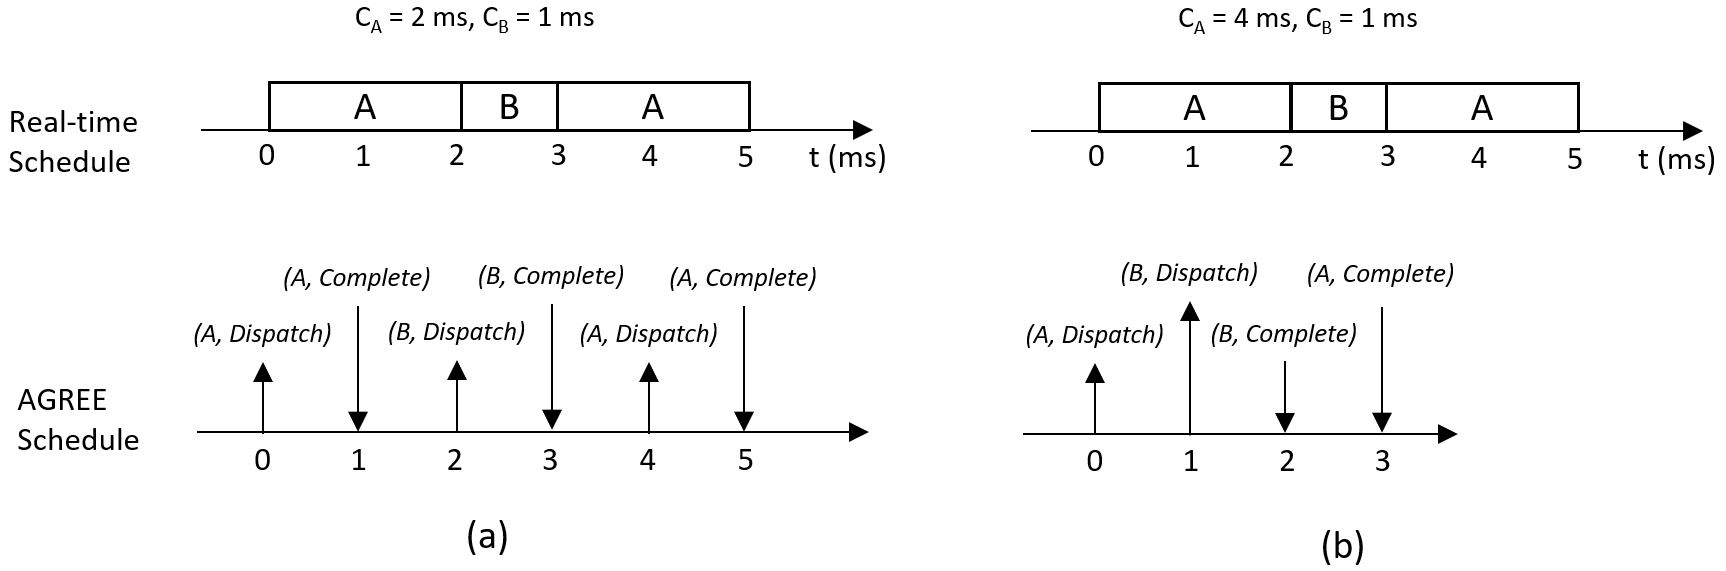
\includegraphics[width=130mm]{RTschedule.jpg}
\caption{Models of Real-Time Schedule in AGREE\label{RTschedule}}
\end{figure}
Given the same real-time schedule, due to the different execution time $C_A$ of $A$, two different AGREE schedules are created. In Figure \ref{RTschedule}(a), since $C_A$ is equal to the time slots assigned to $A$, the end of the each time slot is modeled as \emph{complete}. In Figure \ref{RTschedule}(b), since the first time slot assigned to $A$ is less than its execution time, the end of the first time slot is interpreted as \emph{preemption}, instead of \emph{complete}.

%The AGREE reasoning framework uses past-time LTL [2], particularly LTL operator $G$ (globally), $H$ (historically), and $Z$ (previous). Given a component with an assume-guarantee pair ($A,P$) and an event pair (\emph{dispatch}, \emph{complete}), the meaning of the contract can be formally represented as a past-time LTL formula $G(H((dispatch \Rightarrow A)) \Rightarrow (complete \Rightarrow P))$. In synchronous AGREE, the two events \emph{collpase} into a single instant at each tick. Thus, we have $G(H(A) \Rightarrow P)$.


